\section{Problem Statement}
\label{sec:problem}

% \textcolor{blue}{First, explain your system model. What is that you want to protect? How do you intend to protect it? And the primitives you need for that. Here you could present an example. Then this is also where you explain your Zer-Trust security architecture. This is what your target is.}

Current research on the overlap of DSE and SoC security is rather sparse, with only a handful of papers being identified. Of those discussed in Section \ref{sec:relatedWorks}, Related Works, many focused on identifying the optimal way to implement a specific, RTL-level solution for a specific vulnerability \cite{liu_hardware_2015, rajmohan_hybrid_2020,mahfuz_x-dfs_2025,linares_design_2021}. Another paper, \cite{gressl_security_2019,gressl_design_2021}, automatically created security constraints based on a variety of known attack solutions, rather than just one. However, none of the identified works co-optimize for security, resource and power utilization, and latency, or assess security from the SoC's system or bus level. An example of the architecture, anomaly detection, and security solutions can be seen in Figure \ref{fig:exampleArch}. This shows an architecture with a processor and two components being made more secure by the addition of an anomaly detection methodology and security features. 

%====================
\begin{figure}[h]
\vspace{-3mm}
\centering
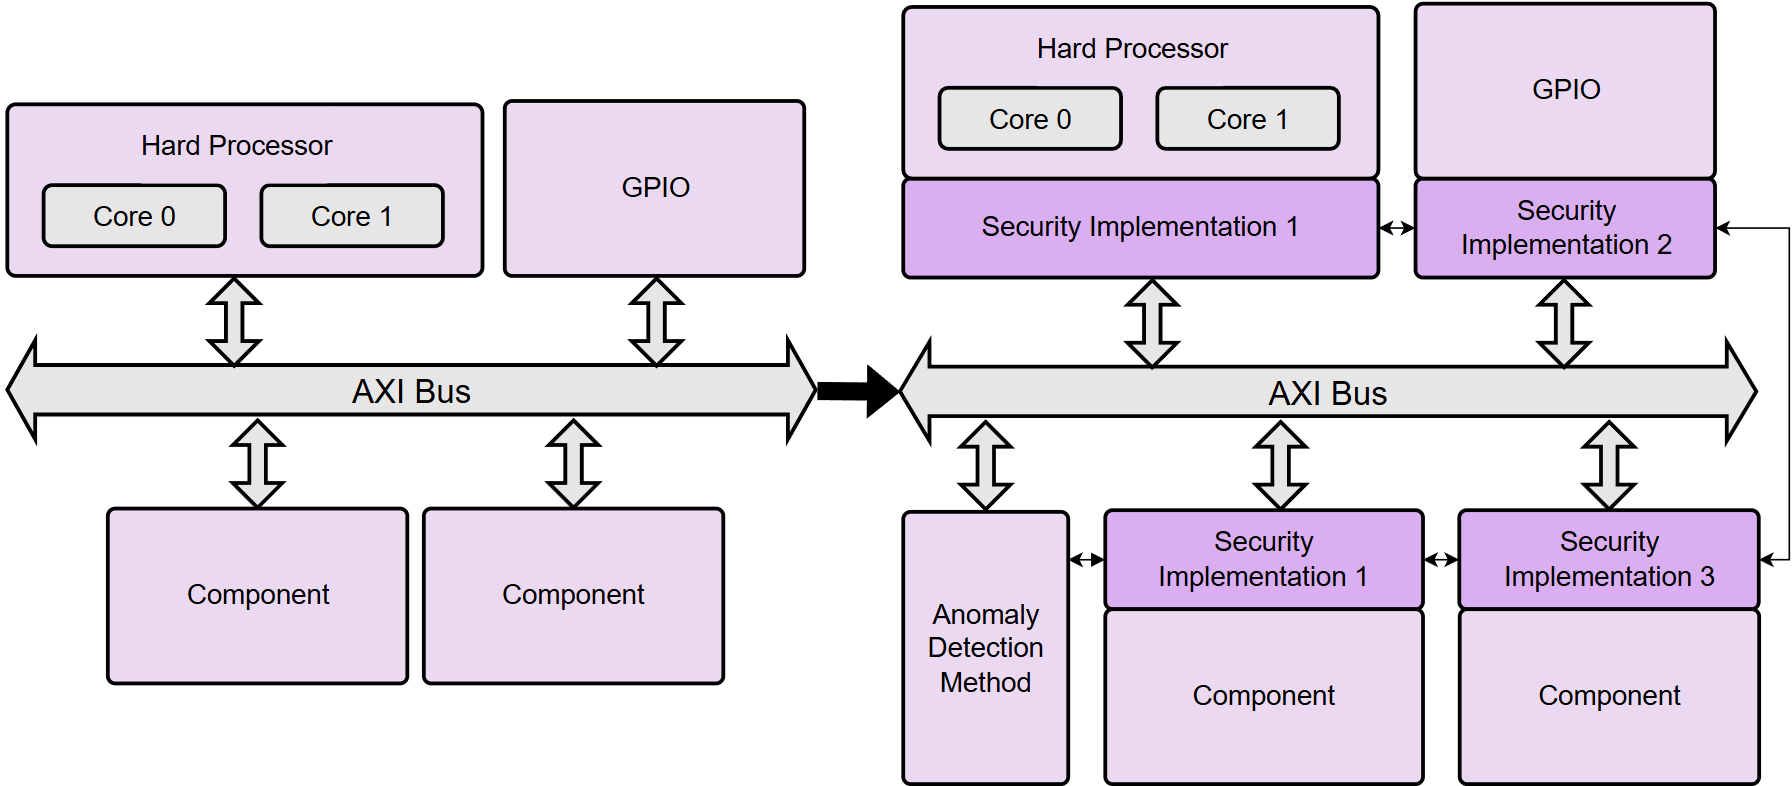
\includegraphics[width=0.5\textwidth]{Images/exampleArch.png}
\caption{\label{fig:exampleArch} Example of a Secured Vs. Unsecured SoC}
\label{figure:SoC_attack}
\vspace{-3mm}
\end{figure}
%====================

This paper aims to generate an optimal SoC implementation from a given specification, addressing various cost functions such as area, power, 
%performance, throughput, latency,
and security. As illustrated in Figure \ref{fig:probspec}, the architecture synthesis process takes the problem specification and produces a secured SoC architecture. This specification can be defined in one of two ways: 1) as a parallel program, or 2) as an abstract SoC architecture.

In the first case, application tasks are allocated to one or more processing components, such as RISC-V, ARM, GPUs, or specialized accelerators. This many-to-many allocation allows multiple tasks to be assigned to multiple processor types. Similarly, data transfers between tasks are allocated to one or more communication components, such as a bus, network-on-chip, or direct link.
In the second case, abstract processors are mapped to concrete processors, and abstract interconnects to physical communication components.

%===================
\begin{figure}[h]
  \centering
  \begin{subfigure}[b]{0.45\textwidth}
    \centering
    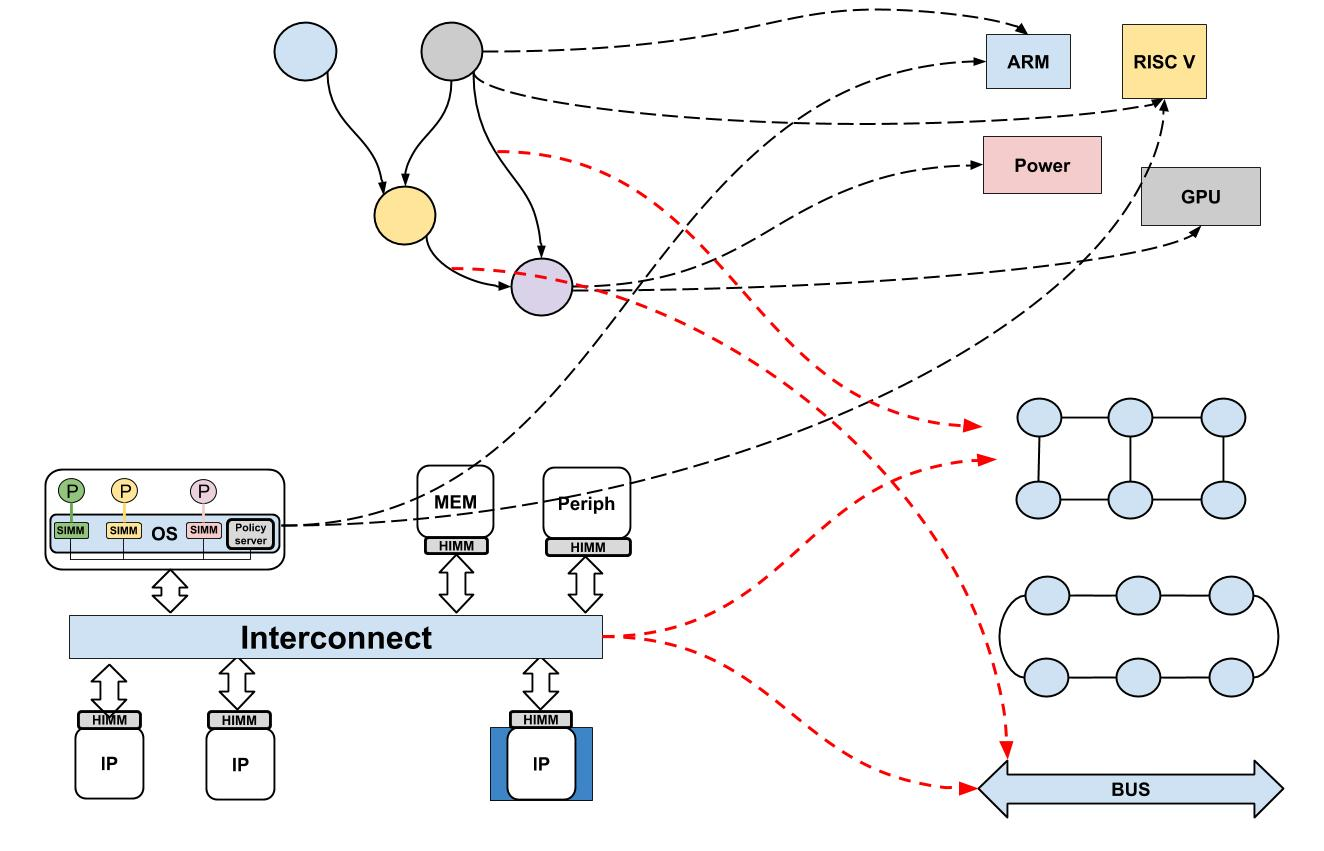
\includegraphics[width=\textwidth]{Images/Secure-SoC-ArchSpec.jpg}
    \caption{Problem Specification}
    \label{fig:probspec}
  \end{subfigure}
  \hspace{0.15cm}
  \begin{subfigure}[b]{0.45\textwidth}
    \centering
    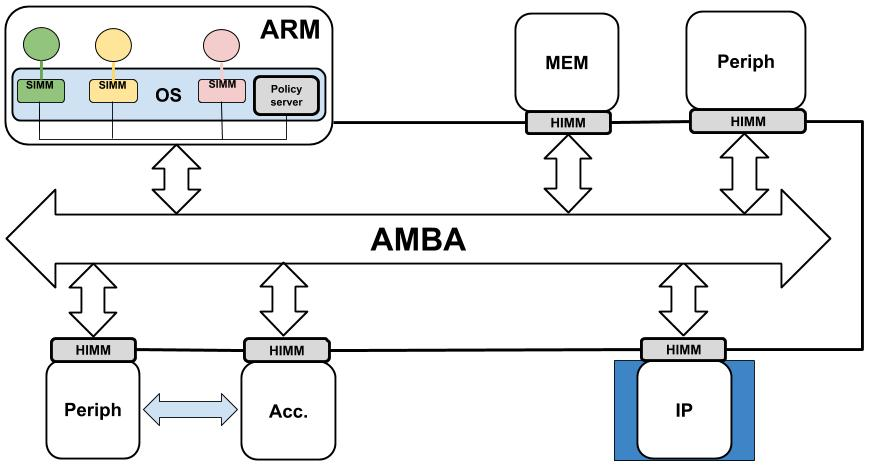
\includegraphics[width=\textwidth]{Images/Secure-SoC-Synthese.jpg}
    \caption{Example of a Concrete Architecture}
    \label{fig:syntharch}
  \end{subfigure}
  \caption{High-Level Synthesis Problem Specification and Optimized Architecture Generation.}
  \label{fig:soc-protection} % caption for the whole figure
\vspace{-3mm}
\end{figure}
%==========================

%\section{Background}
%\label{sec:background}
%\subsection{Design-Space Exploration}
The specific problem addressed in this paper is a multi-objective optimization problem, where multiple, potentially conflicting, goals must be optimized simultaneously.

Multi-objective optimization problems are commonly solved today using Design Space Exploration (DSE), a systematic approach widely adopted in the design of embedded systems and SoCs. DSE seeks configurations that satisfy a set of objectives such as system cost, power consumption, latency, and data throughput, while constraints ensure feasibility and compliance with the target hardware.

DSE identifies optimal designs by evaluating available configurations and analyzing the trade-offs between competing objectives. Applications of DSE include system synthesis, where a system is described as a set of tasks that must be mapped to hardware resources, optimally routed to meet latency targets, and scheduled to respect dependency constraints.



\subsubsection{Specification of SoC Optimization with Security Objectives}

% To consider security as an optimization objective, a means of quantification is necessary. Risk, a common metric for quantifying security, particularly in SoCs \cite{saha_metrics_2022, butka_measuring_2025}, will be used for this purpose in this paper. The following equations formalize risk evaluation.

% \begin{equation}
% \label{eq:ZTARiskWrite}
% R_{Write} = I_{Write} * V_{Write}*L_{Write}
% \end{equation}
% \begin{equation}
% \label{eq:ZTARiskRead}
% R_{Read} = I_{Read} * V_{Read}*L_{Read}
% \end{equation}

% In these equations, the risk \(R\) is calculated for every asset's integrity and confidentiality operations. Each asset has a read risk \(R_{Read}\) and write risk \(R_{Write}\), capturing the two main access methods that can be exploited. 

To optimize System-on-Chip (SoC) designs with security in mind, a quantifiable metric is required. Consistent with prior works \cite{saha_metrics_2022, butka_measuring_2025}, this paper adopts risk as the security objective function, evaluated separately for read and write operations on each exploitable asset, alternatively, integrity and confidentiality.

From \cite{butka_measuring_2025}, the term impact \(I\) refers to the consequence of a successful compromise of the asset. Vulnerability \(V\) refers to the protection level provided by each asset's access controls. Logging capabilities \(L\) assess the presence and responsiveness of logging and anomaly detection mechanisms. Each variable is scored via a custom rubric: \(I\) and \(V\) range from 1-5, and \(L\) from 0.5-2, where lower values indicate stronger security. These values are combined multiplicatively, yielding risk scores from 0.5 to 50. %The maximum value is a risk of 50, and the lowest is 0.5.
At the component level, integrity and confidentiality risks are defined by taking the maximum corresponding risk across all associated assets. This approach ensures that even a single high-risk asset can elevate the component’s overall risk, aligning with conservative design principles. The resulting scores are used programmatically to guide secure design decisions.
%====================
%\begin{wrapfigure}{r}
\begin{figure}[hbt]
% \vspace{-5mm}
\centering
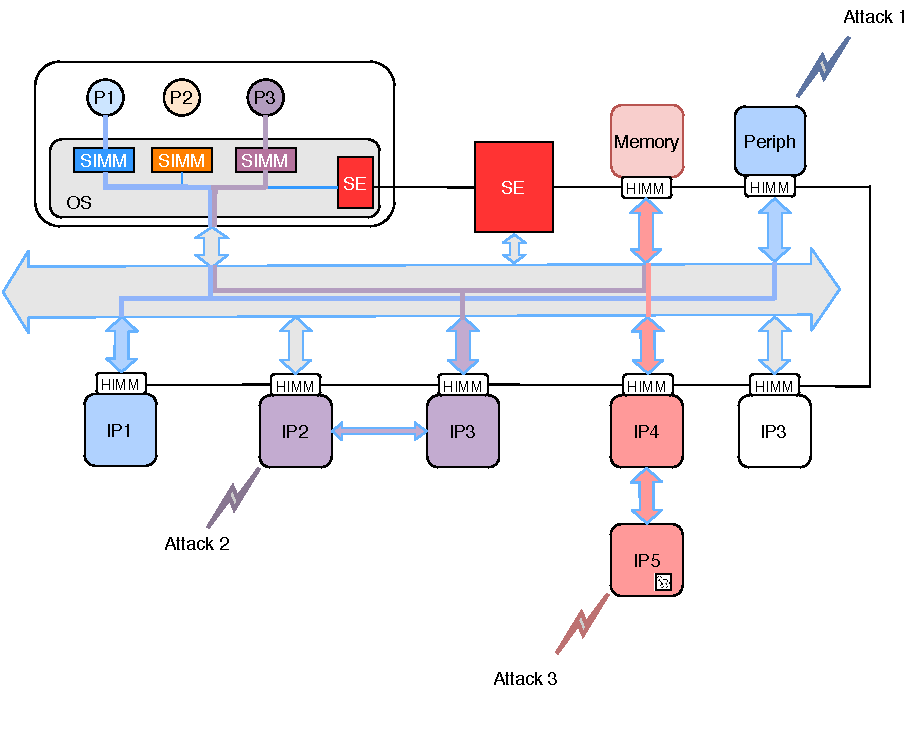
\includegraphics[width=0.48\textwidth]{Images/SoC_attack.pdf}
\vspace{-5mm}

\caption{\label{fig:SoC_attack} Possible Attack Scenarios in a SoC}
\label{figure:SoC_attack}
\vspace{-5mm}
\end{figure}
% \vspace{-5mm}
%\end{wrapfigure}

Figure \ref{figure:SoC_attack} shows a System-on-Chip with three possible attack scenarios. \textbf{Attack 1} targets the SoC's peripheral, impacting IP1 and compromising process P1. \textbf{Attack 2} is a side-channel attack on IP2 that affects IP3 and compromises both memory data and process P3. \textbf{Attack 3} is a HW Trojan attack on IP5 that affects IP4 and compromises memory data. The severity of service disruptions or memory leaks can be quantified by calculating the system's risk factor, which is based on the risk factors of the affected components.
Security evaluation is conducted by assigning risk scores to each system component (processor, IP and interconnect) based on their exploitable assets, access control mechanisms, and threat exposure. It is assumed that each component's designer is best suited to provide security properties, including the asset, attack surface, and potential threats. % The risk factor, which measures the security level, will be calculated based on these values.

To find the impact of an attack on a hardware asset, the SoC and its services are represented as an impact dependency graph. Each process executes by using a combination of functions and hardware assets, and each hardware asset performs a specific function. These hardware assets, required by processes, can be compromised or interrupted by an attack.


\subsection{Answer Set Programming}
Answer Set Programming (ASP) \cite{lifschitz02answerset} is a form of declarative programming oriented towards difficult, primarily NP-hard, search and optimization problems. Rather than describing an algorithm step-by-step, ASP allows for complex problems to be represented as logic programs, which model the problem's functionality. 
ASP specifies what constitutes a valid solution through logical constraints and what makes one solution preferable to another through optimization statements. The solver then searches for all valid solutions, or answer sets, that satisfy constraints and meet optimization objectives. 
The ASP modeling language used in this paper is the Potsdam Answer Set Solving Collection (Potassco) \cite{gebser_potassco_2011}, which can utilize current answer set solvers, such as clingo. 

ASP consists of facts, rules, constraints, and optimization statements. Facts are basic statements about the target architecture, like a component c1, \mintinline[breaklines]{prolog}{component(c1)}, contains three assets \mintinline[breaklines]{prolog}{asset(c1, a1; a2; a3)}. Rules define the relationships between those facts, such as only 1 security solution can be selected per asset \mintinline[breaklines]{prolog}{1{sel_scrty(A,S):scrty_sol(S)}1:-asset(A)}.
Constraints eliminate unwanted solutions by specifying conditions that must not be true, i.e., the total LUT utilization must exceed the maximum available LUTs \mintinline[breaklines]{prolog}{:- ttl_lut_usage(C,TtlLut),TtlLut>max_luts}. 

After identifying all valid solutions that meet constraints, Potassco reports each solution from best to worst, based on the target optimization objective. Optimizations minimize or maximize a value; in this paper, the goal is to minimize system risk  \mintinline[breaklines]{prolog}{#min{Risk,A:asset_risk(A, Action, {Risk)}}}. Therefore, the best solutions report back the smallest system risks, and the worst solutions, the highest.

To bring these concepts together, for example, consider the calculation and minimization of asset risk performed in the proposed design automation for SoC security. First, a function asset\_risk is defined to calculate risk for each asset's integrity and confidentiality risk using a rule.


\begin{minted}[mathescape,
               linenos,
               breaklines,
               breakanywhere,
               numbersep=5pt,
               fontsize=\small,
               frame=lines,
               framesep=2mm,
               style=trac]{prolog}
asset_risk(Asset, Action, Risk) :-
    asset(_, Asset, Action),
    selected_security(Asset, Security),
    selected_logging(Asset, LogFeature),
    vulnerability(Security, Vulnerability),
    logging(LogFeature, LogFactor),
    impact(Asset, Action, Impact),
    Risk = Impact * Vulnerability * LogFactor.
\end{minted}

Where the formal equation this code is based on is represented as:
\begin{equation}
\label{eq:Risk}
\text{Risk}(R) =\text{Impact}(R) \times \text{Vulnerability}(S) \times \text{LogFactor}(L)
\end{equation}

Next, the code ensures that the risk for each asset does not exceed the maximum allowable risk using a constraint. It then performs a minimize function, or optimization, to tell the ASP solver that this value must be minimized as much as possible.


\begin{minted}[mathescape,
               linenos,
               breaklines,
               breakanywhere,
               numbersep=5pt,
               fontsize=\small,
               frame=lines,
               framesep=2mm,
               style=trac]{prolog}
:- asset_risk(_, _, Risk), system_capability(max_asset_risk, MaxRisk), Risk > MaxRisk.
#minimize { Risk, Asset : asset_risk(Asset, Action, Risk) }.
\end{minted}
Where the formal equations these two lines of code are based on are represented as:

\begin{equation}
\label{eq:EnsureLessThanMaxRisk}
\text{asset\_risk}(A) \leq \text{system\_capability}(\text{max\_asset\_risk})
\end{equation}

\begin{equation}
\label{eq:minimizeRisk}
\text{optimization: } \min \sum_{Assets} \text{Risk}(Assets)
\end{equation}

When combined with the rest of the ASP code, this will automatically calculate each asset's risk, ensure it is within the user's maximum risk constraint, and then minimize risk to the lowest possible value. The full ASP code for this paper can be found on the attached GitHub. 

The choice of ASP over alternate solutions such as Integer Linear Programming (ILP) must also be addressed. The core reasoning for using ASP is because of its capability to model complex SoC architectures and interconnects in a clear, readable manner. In their thesis, Surlemont \cite{surlemont_solving_2020} showed that ASP and ILP perform similarly, with minor differences such as ILP outperforming ASP on randomly generated graphs and ASP outperforming ILP on both grid graphs and densely interconnected graphs. As a result, the decision to use ASP comes down to clarity in implementation and formalization. 
